\section{Methodology}
\label{sec:meth}


\subsection{Description of the data}
De dataset die gebruikt gaat worden om deze vragen te beantwoorden is een verzameling van troonredes sinds 1814. Deze troonredes zijn terug te vinden op www.troonredes.nl~\citep{troonredes} . Om een duidelijker beeld te geven van wat de troonrede nu precies is eerst een kleine introductie van wat de troonredes nu precies zijn. 

De troonrede wordt jaarlijks door de koning(in) uitgesproken op Prinsjesdag \todo{waar, voor wie, hoe komt de rest van het land de toespraak ter ore?}. De eerste troonrede werd in 1818 als een algehele toespraak voor de Staten-generaal gehouden. De troonredes worden vooral gebruikt om wets- en beleidsveranderingen door te geven en als beschouwing op het afgelopen jaar en de staat van het land. \todo{referenties graag} In recentere jaren heeft deze beschouwing zich ook uitgebreid naar gebeurtenissen door de hele wereld die invloed uitoefenen op de Nederlandse staat. Sinds 1848 worden de troonredes geschreven door ministers \todo{je kunt hier best wat meer over vertellen} en is het kabinet verantwoordelijk voor de uitspraken. Dit zorgt ervoor dat de troonredes een beeld geven van wat de Nederlandse regering op dat moment belangrijk vindt.

\todo{maak dit subsubsections van de "description of the data"}
\subsection{Missing data}
Er zijn verscheidene jaren waarvan er geen data beschikbaar is, dit doordat er niet elk jaar een troonrede gegeven is. Dit heeft verschillende redenen, zoals oorlogen, angst voor rellen, onvrede over het kabinet of gezondheidsredenen omtrent de koning(in). Dit zorgt ervoor dat niet elk jaar sinds 1818 wordt gerepresenteerd door een troonrede. Omdat de inhoud van de troonredes als verzamelde dataset wordt gebruikt heeft dit minimaal invloed op de uiteindelijke uitkomsten van het onderzoek dat er jaren missen. Door de missende jaren is het weergeven van de verschuiving in onderwerpen mogelijk niet volledig representatief, omdat er geen uitspraken gedaan kunnen worden over de missende jaren.
\todo{geef een lijstje met de missende jaren en geef aan waarom ze dan missen}


\subsection{Quality of the data}
Hier moet nog een deel komen over het feit of het ingescand is of ingetypt.

\pagebreak
\subsection{Wat plotjes en tabelletjes}

Zie het IPython Notebook voor de code om vanuit pandas een poltje op te slaan en een dataframe als tabel op te slaan. Het werkt ideaal! 

De interrupties van Wilders staan beschreven in Figure~\ref{fig:wilders} en Tabel~~\ref{tab:Wilders}.



%\begin{figure}
%\begin{center}
%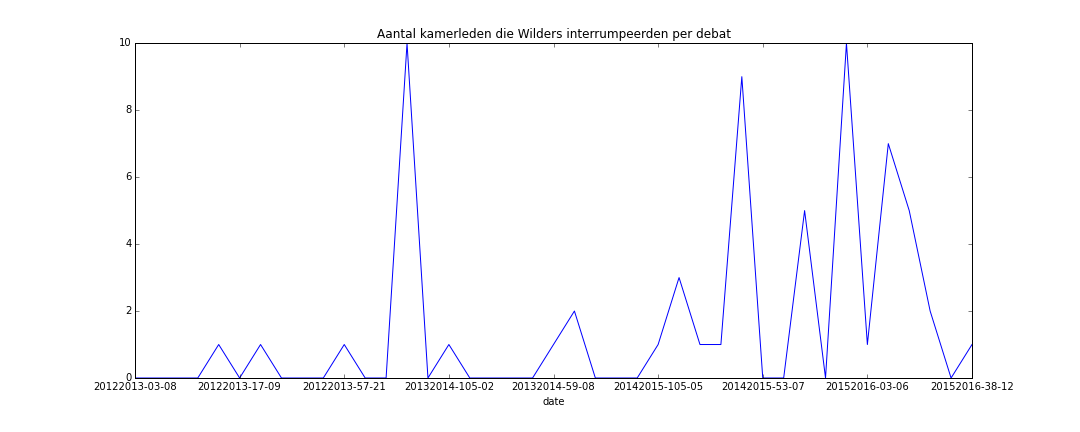
\includegraphics[width=\linewidth]{fig/WildersPlot.png}
%\caption{\label{fig:wilders} Aantal interrupties van Wilders in de Tweede Kamer door de tijd (periode 2012-2016).}
%\end{center}
%\end{figure}


\pagebreak

%\begin{table}[h]
%\begin{footnotesize}
%\begin{tabular}{lrl}
\toprule
{} &  indegree &                               interruptie\_volgorde \\
date            &           &                                                    \\
\midrule
20122013-03-08  &         0 &                                                    \\
20122013-07-16  &         0 &                                                    \\
20122013-100-03 &         0 &                                                    \\
20122013-100-06 &         0 &                                                    \\
20122013-17-06  &         1 &                         Pechtold-Pechtold-Pechtold \\
20122013-17-09  &         0 &                                                    \\
20122013-21-04  &         1 &                         Pechtold-Pechtold-Pechtold \\
20122013-22-08  &         0 &                                                    \\
20122013-32-06  &         0 &                                                    \\
20122013-48-23  &         0 &                                                    \\
20122013-57-21  &         1 &  Pechtold-Pechtold-Pechtold-Pechtold-Pechtold-P... \\
20122013-76-03  &         0 &                                                    \\
20122013-76-06  &         0 &                                                    \\
20132014-05-02  &        10 &  Roemer-Roemer-Van Haersma Buma-Van Haersma Bum... \\
20132014-06-04  &         0 &                                                    \\
20132014-105-02 &         1 &  Pechtold-Pechtold-Pechtold-Pechtold-Pechtold-P... \\
20132014-105-06 &         0 &                                                    \\
20132014-14-03  &         0 &                                                    \\
20132014-14-06  &         0 &                                                    \\
20132014-52-18  &         0 &                                                    \\
20132014-59-08  &         1 &                               Klaver-Klaver-Klaver \\
20142015-02-08  &         2 &  Pechtold-Pechtold-Pechtold-Pechtold-Pechtold-P... \\
20142015-03-06  &         0 &                                                    \\
20142015-09-09  &         0 &                                                    \\
20142015-100-05 &         0 &                                                    \\
20142015-105-05 &         1 &                                  Pechtold-Pechtold \\
20142015-111-04 &         3 &  Pechtold-Pechtold-Pechtold-Pechtold-Pechtold-P... \\
20142015-111-07 &         1 &                                  Pechtold-Pechtold \\
20142015-39-71  &         1 &                                  Pechtold-Pechtold \\
20142015-41-07  &         9 &  Samsom-Samsom-Pechtold-Pechtold-Pechtold-Kuzu-... \\
20142015-53-07  &         0 &                                                    \\
20142015-61-23  &         0 &                                                    \\
20142015-79-07  &         5 &  Klaver-Klaver-Klaver-Gesthuizen-Gesthuizen-Ges... \\
20142015-95-06  &         0 &                                                    \\
20152016-02-07  &        10 &  Pechtold-Pechtold-Pechtold-Pechtold-Slob-Slob-... \\
20152016-03-06  &         1 &       Pechtold-Pechtold-Pechtold-Pechtold-Pechtold \\
20152016-14-02  &         7 &  Klaver-Klaver-Roemer-Roemer-Roemer-Roemer-Sams... \\
20152016-14-05  &         5 &  Van Haersma Buma-Van Haersma Buma-Van Haersma ... \\
20152016-27-03  &         2 &  Segers-Segers-Segers-Segers-Kuzu-Kuzu-Kuzu-Kuz... \\
20152016-38-10  &         0 &                                                    \\
20152016-38-12  &         1 &                                        Klein-Klein \\
\bottomrule
\end{tabular}

%\end{footnotesize}
%\caption{\label{tab:Wilders} Door wie werd Wilders onderbroken en hoe vaak per debat.}
%\end{table}


\pagebreak
\subsection{Methods}
Het gehele corpus bestaat uit 117 verschillende troonredes, welke in totaal uit 143875 woorden bestaan. \todo{die vorige zin hoort toch in description of the data?}
Om uit deze data te kunnen achterhalen of er overkoepelende thema's/onderwerpen zijn en wat deze mogelijk zijn wordt er gebruik gemaakt van tekstanalyse technieken. Specifiek wordt er gebruik gemaakt van co-occurence aanpakken.~\cite{callon1991co} Hierbij worden categoriën geinduceerd door te kijken naar het samen voorkomen van termen in afzonderlijke stukken tekst.\todo{Leg eerst veel meer uit wat die techniek inhoudt voor je hem gaat aanprijzen. De precieze uitleg is belangrijker, en ook leuker om te schrijven }
 Hierbij is het doel om uit te vinden welke termen relevant zijn en hoe deze zich over tijd met andere termen associëren. Met behulp van deze informatie zouden er uitspraken gedaan kunnen worden over de onderwerpen die termen impliceren. Hiermee kunnen dan uitspraken worden gedaan over de inhoud van een specifieke troonrede aan de hand van de termen in de tekst. 

Voordat deze uitspraken echter kunnen worden gedaan moet de data eerst worden verwerkt zodat er analyse op kan worden gedaan. Hiervoor worden de teksten van de troonredes eerst gelemmatiseerd. Hierdoor worden de woorden herleid tot hun lemma(stam), waardoor ze kunnen worden geanalyseerd als één term. \todo{Denk je dat je moeder nu zou snappen wat je doet? Ik niet. Terwijl ze precies weet wat hier gebeurt. Dus leg het echt goed uit, en leg ook goed uit \em{waarom} je dit zo graag doet. } Met behulp van deze gelemmatiseerde termen wordt een co-occurence matrix opgesteld. Deze matrix omvat voor alle combinaties van termen \todo{onduidelijk/vaag} de frequentie dat ze samen in een paragraaf voorkomen. 

Voor alle combinaties uit deze matrix wordt een nabijheidsscore berekend via het volgende algoritme. \todo{Dit is geen algoritme.} \todo{Definieer eerst PMI (jij noemt dat I), en maak een referentie naar pointwise mutual information. Je kunt het ook rustig uitleggen met een voorbeeld. Ook zou je kunen uitleggen wat PMI "doet"/betekent. Denk maar terug aan jezelf: je hebt er echt mee geworsteld. Dus je kunt het nu goed uitleggen!}

 $$S(W_1,W_2)=\frac{\sum_{c\epsilon W\{W_1,W_2\},I(W_1,c)>0}min(I(W_1,c),I(W_2,c))}{\sum_{c\epsilon W\{W_1,W_2\},I(W_1,c)>0}I(W_1,c)}$$ Dit algoritme maakt gebruik van de woorden uit het gehele corpus om context te bepalen. Hiervoor wordt voor elke combinatie woorden (W1,W2) gekeken naar de woorden waarmee ze
samen in een paragraaf voorkomen. De som van I(W,C) voor alle woorden (C) uit het corpus waarvoor geldt dat I(W,C) > 0 wordt voor beide woorden berekend. Als hieruit volgt dat I(W,C) voor beide woorden gelijk is kan men stellen dat als W1 in een paragraaf voorkomt W2 ook voorkomt en vice versa. Een verwantschapsscore van 0 geeft aan dat de woorden nooit samen in een paragraaf voorkomen. Aan de hand van deze score wordt een gewogen semantisch netwerk gevormd met de termen als nodes en de gewichten op de edges. Om de termen binnen dit netwerk te kunnen analyseren wordt gebruik gemaakt van een community detectie algoritme. Het specifieke algoritme dat gebruikt wordt is dat van~\cite{blondel2008fast}. Het doel van dit algoritme is om vanuit het gewogen netwerk clusters te vormen van samenhangende subsets van termen. Afhankelijk van de termen binnen deze
clusters kunnen deze clusters gezien worden als indicatief voor onderwerpen/thema's binnen het corpus. Dit induceren van onderwerpen moet een overzicht geven van de verschillende termen die tot  een onderwerp behoren en hoe sterk de samenhang is tussen termen binnen een onderwerp. Ook zou het een beeld moeten geven van de samenhang tussen verschillende onderwerpen. 
\\
Om tot het gewogen netwerk te komen dat gebruikt kan worden voor de clustering wordt de dataset van woorden binnen het gehele corpus eerst gereduceerd tot de meest relevante data. Allereerst wordt de dataset gelemmatiseerd, waarna de 1000 meest voorkomende termen gebruikt worden om de co-occurence matrix op te stellen. De nabijheidsscore voor de termen uit deze matrix worden berekend en om ervoor te zorgen dat enkel de meest relevante termen worden meegegeven aan het community detectie algoritme wordt een drempel bepaald. Deze drempel geeft aan vanaf welke waarde van de nabijheidsscore de co-occurence combinaties door het algoritme verwerkt worden. De drempelwaarde ligt tussen de 0 en 1 en wordt bepaald door vanaf 0 de score telkens op te hogen. De drempelwaarde is bereikt als er binnen het netwerk een component van meer dan 2 nodes verdwijnt. Hiermee worden de zwak verbonden nodes uit het netwerk verwijderd. De drempelwaarde die gevonden is voor ons netwerk is θ=0.65. Het resulterende netwerk is door het community detectie algoritme verwerkt om de verschillende subsets te kunnen identificeren. Vanuit deze subsets wordt bepaald aan de hand van de termen die er onder vallen of er een onderwerp mee geassocieerd kan worden.


\subsubsection{RQ1}

\subsubsection{RQ2}